\documentclass[10pt]{article}
% Preambulo compartido por los entregables escritos de Diablos AeroVision (HACK-018).
% Compila con pdflatex (TeX Live, MiKTeX u Overleaf). Ver docs/latex/README.md.
\usepackage[T1]{fontenc}
\usepackage[utf8]{inputenc}
\usepackage[spanish,es-noshorthands,es-tabla,es-nodecimaldot]{babel}
\usepackage{lmodern}
\usepackage{microtype}
\usepackage[a4paper,margin=2.2cm]{geometry}
\usepackage{amsmath,amssymb}
\usepackage{booktabs}
\usepackage{tabularx}
\usepackage{graphicx}
\usepackage{float}
\usepackage{enumitem}
\usepackage[table]{xcolor}
\usepackage{caption}
\usepackage{fancyhdr}
\usepackage[hidelinks]{hyperref}

\definecolor{diablos}{HTML}{B3121B}
\definecolor{grisfondo}{HTML}{F4F4F5}
\captionsetup{font=small,labelfont=bf}
\setlist{itemsep=2pt,topsep=4pt}
\setlength{\parskip}{4pt}

% \cf{clave}: cifra leida de reports/ via generated/cifras.tex. Una clave inexistente
% se imprime en rojo para que nunca pase inadvertida (y el test la rechaza).
\makeatletter
\newcommand{\cf}[1]{\@ifundefined{cf@#1}{\textcolor{red}{\textbf{??#1}}}{\@nameuse{cf@#1}}}
\makeatother
% ARCHIVO GENERADO por analysis/build_paper_numbers.py. No editar a mano.
\makeatletter
\@namedef{cf@ca.changeup.sc}{91.5}
\@namedef{cf@ca.changeup.sd}{\ensuremath{-}0.51}
\@namedef{cf@ca.changeup.sd.abs}{0.51}
\@namedef{cf@ca.changeup.sn}{92.0}
\@namedef{cf@ca.changeup.uso}{28}
\@namedef{cf@ca.slider.sc}{96.8}
\@namedef{cf@ca.slider.sd}{+0.20}
\@namedef{cf@ca.slider.sd.abs}{0.20}
\@namedef{cf@ca.slider.sn}{96.6}
\@namedef{cf@ca.slider.uso}{72}
\@namedef{cf@ca1.ct}{+0.85}
\@namedef{cf@ca1.ct.abs}{0.85}
\@namedef{cf@ca1.gb}{59}
\@namedef{cf@ca1.id}{pitcher\_00778}
\@namedef{cf@ca1.ln}{102.1}
\@namedef{cf@ca1.mano}{zurdo}
\@namedef{cf@ca1.n}{1,177}
\@namedef{cf@ca1.pc}{100.6}
\@namedef{cf@ca1.pn}{101.5}
\@namedef{cf@ca1.rank.delta}{5}
\@namedef{cf@ca1.rank.sn}{423}
\@namedef{cf@ca1.rp}{+1.02}
\@namedef{cf@ca1.rp.abs}{1.02}
\@namedef{cf@ca1.sc}{96.1}
\@namedef{cf@ca1.sd}{+0.31}
\@namedef{cf@ca1.sd.abs}{0.31}
\@namedef{cf@ca1.slot}{33}
\@namedef{cf@ca1.sn}{95.8}
\@namedef{cf@ca1.velo}{82.7}
\@namedef{cf@ca1.year}{2024}
\@namedef{cf@ca2.ct}{+1.45}
\@namedef{cf@ca2.ct.abs}{1.45}
\@namedef{cf@ca2.gb}{74}
\@namedef{cf@ca2.id}{pitcher\_00778}
\@namedef{cf@ca2.ln}{102.3}
\@namedef{cf@ca2.mano}{zurdo}
\@namedef{cf@ca2.n}{1,280}
\@namedef{cf@ca2.pc}{100.3}
\@namedef{cf@ca2.pn}{101.3}
\@namedef{cf@ca2.rank.delta}{11}
\@namedef{cf@ca2.rank.sn}{432}
\@namedef{cf@ca2.rp}{+0.10}
\@namedef{cf@ca2.rp.abs}{0.10}
\@namedef{cf@ca2.sc}{95.3}
\@namedef{cf@ca2.sd}{+0.00}
\@namedef{cf@ca2.sd.abs}{0.00}
\@namedef{cf@ca2.slot}{34}
\@namedef{cf@ca2.sn}{95.3}
\@namedef{cf@ca2.velo}{81.8}
\@namedef{cf@ca2.year}{2025}
\@namedef{cf@cal.max.global}{0.022}
\@namedef{cf@cal.stuff.park.mean}{0.0105}
\@namedef{cf@canal.n}{778}
\@namedef{cf@canal.park}{\ensuremath{-}0.0060}
\@namedef{cf@canal.park.abs}{0.0060}
\@namedef{cf@canal.park.ci}{[\ensuremath{-}0.0079, \ensuremath{-}0.0040]}
\@namedef{cf@canal.park.per100}{\ensuremath{-}0.60}
\@namedef{cf@canal.park.per100.abs}{0.60}
\@namedef{cf@canal.park.share}{42}
\@namedef{cf@canal.ratio}{4.7}
\@namedef{cf@canal.stuff}{\ensuremath{-}0.0013}
\@namedef{cf@canal.stuff.abs}{0.0013}
\@namedef{cf@canal.stuff.ci}{[\ensuremath{-}0.0013, \ensuremath{-}0.0012]}
\@namedef{cf@canal.stuff.per100}{\ensuremath{-}0.13}
\@namedef{cf@canal.stuff.per100.abs}{0.13}
\@namedef{cf@canal.stuff.share}{9}
\@namedef{cf@canal.total}{\ensuremath{-}0.0141}
\@namedef{cf@canal.total.abs}{0.0141}
\@namedef{cf@canal.total.ci}{[\ensuremath{-}0.0169, \ensuremath{-}0.0117]}
\@namedef{cf@canal.total.per100}{\ensuremath{-}1.41}
\@namedef{cf@canal.total.per100.abs}{1.41}
\@namedef{cf@canal.total.share}{100}
\@namedef{cf@canal.unallocated}{\ensuremath{-}0.0069}
\@namedef{cf@canal.unallocated.abs}{0.0069}
\@namedef{cf@canal.unallocated.ci}{[\ensuremath{-}0.0086, \ensuremath{-}0.0052]}
\@namedef{cf@canal.unallocated.per100}{\ensuremath{-}0.69}
\@namedef{cf@canal.unallocated.per100.abs}{0.69}
\@namedef{cf@canal.unallocated.share}{48}
\@namedef{cf@cb.ct}{+2.49}
\@namedef{cf@cb.ct.abs}{2.49}
\@namedef{cf@cb.fourseam.sc}{95.3}
\@namedef{cf@cb.fourseam.sd}{\ensuremath{-}9.03}
\@namedef{cf@cb.fourseam.sd.abs}{9.03}
\@namedef{cf@cb.fourseam.sn}{104.3}
\@namedef{cf@cb.fourseam.uso}{77}
\@namedef{cf@cb.gb}{56}
\@namedef{cf@cb.id}{pitcher\_00204}
\@namedef{cf@cb.ln}{99.1}
\@namedef{cf@cb.mano}{zurdo}
\@namedef{cf@cb.n}{658}
\@namedef{cf@cb.pc}{98.5}
\@namedef{cf@cb.pctl}{97}
\@namedef{cf@cb.pn}{100.2}
\@namedef{cf@cb.rank.delta}{461}
\@namedef{cf@cb.rank.sn}{13}
\@namedef{cf@cb.rp}{+1.05}
\@namedef{cf@cb.rp.abs}{1.05}
\@namedef{cf@cb.sc}{99.5}
\@namedef{cf@cb.sd}{\ensuremath{-}6.99}
\@namedef{cf@cb.sd.abs}{6.99}
\@namedef{cf@cb.sinker.sc}{102.0}
\@namedef{cf@cb.sinker.sd}{\ensuremath{-}1.40}
\@namedef{cf@cb.sinker.sd.abs}{1.40}
\@namedef{cf@cb.sinker.sn}{103.4}
\@namedef{cf@cb.sinker.uso}{0}
\@namedef{cf@cb.slider.sc}{113.8}
\@namedef{cf@cb.slider.sd}{\ensuremath{-}0.05}
\@namedef{cf@cb.slider.sd.abs}{0.05}
\@namedef{cf@cb.slider.sn}{113.9}
\@namedef{cf@cb.slider.uso}{22}
\@namedef{cf@cb.slot}{41}
\@namedef{cf@cb.sn}{106.4}
\@namedef{cf@cb.velo}{93.5}
\@namedef{cf@cb.year}{2025}
\@namedef{cf@cc.canalparquebip}{\ensuremath{-}1.86}
\@namedef{cf@cc.canalparquebip.abs}{1.86}
\@namedef{cf@cc.canaltotal}{\ensuremath{-}4.41}
\@namedef{cf@cc.canaltotal.abs}{4.41}
\@namedef{cf@cc.changeup.sc}{105.1}
\@namedef{cf@cc.changeup.sd}{\ensuremath{-}1.68}
\@namedef{cf@cc.changeup.sd.abs}{1.68}
\@namedef{cf@cc.changeup.sn}{106.8}
\@namedef{cf@cc.changeup.uso}{16}
\@namedef{cf@cc.ct}{\ensuremath{-}4.41}
\@namedef{cf@cc.ct.abs}{4.41}
\@namedef{cf@cc.curveball.sc}{107.6}
\@namedef{cf@cc.curveball.sd}{+0.29}
\@namedef{cf@cc.curveball.sd.abs}{0.29}
\@namedef{cf@cc.curveball.sn}{107.3}
\@namedef{cf@cc.curveball.uso}{11}
\@namedef{cf@cc.fourseam.sc}{90.3}
\@namedef{cf@cc.fourseam.sd}{\ensuremath{-}9.77}
\@namedef{cf@cc.fourseam.sd.abs}{9.77}
\@namedef{cf@cc.fourseam.sn}{100.1}
\@namedef{cf@cc.fourseam.uso}{73}
\@namedef{cf@cc.gb}{46}
\@namedef{cf@cc.id}{pitcher\_00466}
\@namedef{cf@cc.ln}{99.8}
\@namedef{cf@cc.mano}{derecho}
\@namedef{cf@cc.n}{868}
\@namedef{cf@cc.pc}{98.7}
\@namedef{cf@cc.pn}{100.6}
\@namedef{cf@cc.rank.delta}{462}
\@namedef{cf@cc.rank.sn}{141}
\@namedef{cf@cc.rp}{+0.15}
\@namedef{cf@cc.rp.abs}{0.15}
\@namedef{cf@cc.sc}{94.5}
\@namedef{cf@cc.sd}{\ensuremath{-}7.40}
\@namedef{cf@cc.sd.abs}{7.40}
\@namedef{cf@cc.slot}{48}
\@namedef{cf@cc.sn}{101.9}
\@namedef{cf@cc.velo}{91.3}
\@namedef{cf@cc.year}{2025}
\@namedef{cf@cf.changeup.cdmx}{101.5}
\@namedef{cf@cf.changeup.delta}{\ensuremath{-}1.6}
\@namedef{cf@cf.changeup.delta.abs}{1.6}
\@namedef{cf@cf.changeup.neutral}{103.1}
\@namedef{cf@cf.curveball.cdmx}{108.2}
\@namedef{cf@cf.curveball.delta}{\ensuremath{-}0.5}
\@namedef{cf@cf.curveball.delta.abs}{0.5}
\@namedef{cf@cf.curveball.neutral}{108.7}
\@namedef{cf@cf.cutter.cdmx}{95.2}
\@namedef{cf@cf.cutter.delta}{\ensuremath{-}0.4}
\@namedef{cf@cf.cutter.delta.abs}{0.4}
\@namedef{cf@cf.cutter.neutral}{95.6}
\@namedef{cf@cf.fourseam.cdmx}{90.9}
\@namedef{cf@cf.fourseam.delta}{\ensuremath{-}4.5}
\@namedef{cf@cf.fourseam.delta.abs}{4.5}
\@namedef{cf@cf.fourseam.neutral}{95.5}
\@namedef{cf@cf.sinker.cdmx}{89.4}
\@namedef{cf@cf.sinker.delta}{\ensuremath{-}2.1}
\@namedef{cf@cf.sinker.delta.abs}{2.1}
\@namedef{cf@cf.sinker.neutral}{91.5}
\@namedef{cf@cf.slider.cdmx}{109.0}
\@namedef{cf@cf.slider.delta}{\ensuremath{-}0.3}
\@namedef{cf@cf.slider.delta.abs}{0.3}
\@namedef{cf@cf.slider.neutral}{109.3}
\@namedef{cf@cf.splitter.cdmx}{107.5}
\@namedef{cf@cf.splitter.delta}{\ensuremath{-}1.3}
\@namedef{cf@cf.splitter.delta.abs}{1.3}
\@namedef{cf@cf.splitter.neutral}{108.7}
\@namedef{cf@datos.juegos}{2,127}
\@namedef{cf@datos.pitcheos}{634,624}
\@namedef{cf@datos.pitchers}{1,135}
\@namedef{cf@diag.loc.excess}{0.13}
\@namedef{cf@diag.loc.r2oos}{0.31}
\@namedef{cf@diag.loc.r2ref}{0.18}
\@namedef{cf@escala.loc.sigma}{0.0742}
\@namedef{cf@escala.pit.sigma}{0.0774}
\@namedef{cf@escala.stuff.punto}{0.00054}
\@namedef{cf@escala.stuff.sigma}{0.0054}
\@namedef{cf@h1.changeup.hr}{+0.09}
\@namedef{cf@h1.changeup.hr.abs}{0.09}
\@namedef{cf@h1.changeup.hrp}{0.52}
\@namedef{cf@h1.changeup.n}{541}
\@namedef{cf@h1.changeup.tib}{\ensuremath{-}4.5}
\@namedef{cf@h1.changeup.tib.abs}{4.5}
\@namedef{cf@h1.changeup.tibabs}{4.5}
\@namedef{cf@h1.changeup.whiff}{\ensuremath{-}1.96}
\@namedef{cf@h1.changeup.whiff.abs}{1.96}
\@namedef{cf@h1.changeup.whiffp}{\ensuremath{<}0.01}
\@namedef{cf@h1.changeup.zs}{+0.89}
\@namedef{cf@h1.changeup.zs.abs}{0.89}
\@namedef{cf@h1.curveball.hr}{+0.38}
\@namedef{cf@h1.curveball.hr.abs}{0.38}
\@namedef{cf@h1.curveball.hrp}{0.28}
\@namedef{cf@h1.curveball.n}{363}
\@namedef{cf@h1.curveball.tib}{\ensuremath{-}3.7}
\@namedef{cf@h1.curveball.tib.abs}{3.7}
\@namedef{cf@h1.curveball.tibabs}{3.7}
\@namedef{cf@h1.curveball.whiff}{\ensuremath{-}0.27}
\@namedef{cf@h1.curveball.whiff.abs}{0.27}
\@namedef{cf@h1.curveball.whiffp}{0.75}
\@namedef{cf@h1.curveball.zs}{+1.05}
\@namedef{cf@h1.curveball.zs.abs}{1.05}
\@namedef{cf@h1.cutter.hr}{+0.18}
\@namedef{cf@h1.cutter.hr.abs}{0.18}
\@namedef{cf@h1.cutter.hrp}{0.62}
\@namedef{cf@h1.cutter.n}{92}
\@namedef{cf@h1.cutter.tib}{\ensuremath{-}2.7}
\@namedef{cf@h1.cutter.tib.abs}{2.7}
\@namedef{cf@h1.cutter.tibabs}{2.7}
\@namedef{cf@h1.cutter.whiff}{+0.88}
\@namedef{cf@h1.cutter.whiff.abs}{0.88}
\@namedef{cf@h1.cutter.whiffp}{0.48}
\@namedef{cf@h1.cutter.zs}{+1.08}
\@namedef{cf@h1.cutter.zs.abs}{1.08}
\@namedef{cf@h1.fourseam.hr}{+0.09}
\@namedef{cf@h1.fourseam.hr.abs}{0.09}
\@namedef{cf@h1.fourseam.hrp}{0.32}
\@namedef{cf@h1.fourseam.n}{642}
\@namedef{cf@h1.fourseam.tib}{\ensuremath{-}4.7}
\@namedef{cf@h1.fourseam.tib.abs}{4.7}
\@namedef{cf@h1.fourseam.tibabs}{4.7}
\@namedef{cf@h1.fourseam.whiff}{\ensuremath{-}1.85}
\@namedef{cf@h1.fourseam.whiff.abs}{1.85}
\@namedef{cf@h1.fourseam.whiffp}{\ensuremath{<}0.01}
\@namedef{cf@h1.fourseam.zs}{+1.35}
\@namedef{cf@h1.fourseam.zs.abs}{1.35}
\@namedef{cf@h1.sinker.hr}{+0.18}
\@namedef{cf@h1.sinker.hr.abs}{0.18}
\@namedef{cf@h1.sinker.hrp}{0.12}
\@namedef{cf@h1.sinker.n}{409}
\@namedef{cf@h1.sinker.tib}{\ensuremath{-}4.8}
\@namedef{cf@h1.sinker.tib.abs}{4.8}
\@namedef{cf@h1.sinker.tibabs}{4.8}
\@namedef{cf@h1.sinker.whiff}{\ensuremath{-}1.07}
\@namedef{cf@h1.sinker.whiff.abs}{1.07}
\@namedef{cf@h1.sinker.whiffp}{0.02}
\@namedef{cf@h1.sinker.zs}{+1.34}
\@namedef{cf@h1.sinker.zs.abs}{1.34}
\@namedef{cf@h1.slider.hr}{+0.16}
\@namedef{cf@h1.slider.hr.abs}{0.16}
\@namedef{cf@h1.slider.hrp}{0.22}
\@namedef{cf@h1.slider.n}{648}
\@namedef{cf@h1.slider.tib}{\ensuremath{-}2.0}
\@namedef{cf@h1.slider.tib.abs}{2.0}
\@namedef{cf@h1.slider.tibabs}{2.0}
\@namedef{cf@h1.slider.whiff}{\ensuremath{-}0.96}
\@namedef{cf@h1.slider.whiff.abs}{0.96}
\@namedef{cf@h1.slider.whiffp}{0.04}
\@namedef{cf@h1.slider.zs}{+0.93}
\@namedef{cf@h1.slider.zs.abs}{0.93}
\@namedef{cf@h1.splitter.hr}{\ensuremath{-}0.11}
\@namedef{cf@h1.splitter.hr.abs}{0.11}
\@namedef{cf@h1.splitter.hrp}{0.75}
\@namedef{cf@h1.splitter.ivbp}{0.18}
\@namedef{cf@h1.splitter.n}{35}
\@namedef{cf@h1.splitter.p}{0.002}
\@namedef{cf@h1.splitter.tib}{\ensuremath{-}3.2}
\@namedef{cf@h1.splitter.tib.abs}{3.2}
\@namedef{cf@h1.splitter.tibabs}{3.2}
\@namedef{cf@h1.splitter.whiff}{\ensuremath{-}2.04}
\@namedef{cf@h1.splitter.whiff.abs}{2.04}
\@namedef{cf@h1.splitter.whiffp}{0.41}
\@namedef{cf@h1.splitter.zs}{+0.51}
\@namedef{cf@h1.splitter.zs.abs}{0.51}
\@namedef{cf@h2.ci}{[0.65, 0.94]}
\@namedef{cf@h2.est}{0.79}
\@namedef{cf@h2.n}{754}
\@namedef{cf@h3.ci}{[\ensuremath{-}0.107, 0.100]}
\@namedef{cf@h3.est}{\ensuremath{-}0.010}
\@namedef{cf@h3.est.abs}{0.010}
\@namedef{cf@h3.hr.est}{\ensuremath{-}0.0015}
\@namedef{cf@h3.hr.est.abs}{0.0015}
\@namedef{cf@h3.hr.p}{0.90}
\@namedef{cf@h3.n}{792}
\@namedef{cf@h3.p}{0.83}
\@namedef{cf@h4.n}{892}
\@namedef{cf@h4.whiff.hb.p}{0.15}
\@namedef{cf@h4.whiff.hb.per100}{0.1809}
\@namedef{cf@h4.whiff.hb.prel}{=0.15}
\@namedef{cf@h4.whiff.ivb.p}{0.47}
\@namedef{cf@h4.whiff.ivb.per100}{\ensuremath{-}0.1859}
\@namedef{cf@h4.whiff.ivb.per100.abs}{0.1859}
\@namedef{cf@h4.whiff.ivb.prel}{=0.47}
\@namedef{cf@h4.whiff.s2b.p}{0.04}
\@namedef{cf@h4.whiff.s2b.per100}{\ensuremath{-}0.3603}
\@namedef{cf@h4.whiff.s2b.per100.abs}{0.3603}
\@namedef{cf@h4.whiff.s2b.prel}{=0.04}
\@namedef{cf@h4.whiff.spin.p}{0.03}
\@namedef{cf@h4.whiff.spin.per100}{0.0032}
\@namedef{cf@h4.whiff.spin.prel}{=0.03}
\@namedef{cf@h4.xrv.hb.p}{0.69}
\@namedef{cf@h4.xrv.hb.per100}{\ensuremath{-}0.0460}
\@namedef{cf@h4.xrv.hb.per100.abs}{0.0460}
\@namedef{cf@h4.xrv.hb.prel}{=0.69}
\@namedef{cf@h4.xrv.ivb.p}{0.31}
\@namedef{cf@h4.xrv.ivb.per100}{\ensuremath{-}0.0977}
\@namedef{cf@h4.xrv.ivb.per100.abs}{0.0977}
\@namedef{cf@h4.xrv.ivb.prel}{=0.31}
\@namedef{cf@h4.xrv.s2b.p}{0.74}
\@namedef{cf@h4.xrv.s2b.per100}{\ensuremath{-}0.0443}
\@namedef{cf@h4.xrv.s2b.per100.abs}{0.0443}
\@namedef{cf@h4.xrv.s2b.prel}{=0.74}
\@namedef{cf@h4.xrv.spin.p}{\ensuremath{<}0.01}
\@namedef{cf@h4.xrv.spin.per100}{0.0028}
\@namedef{cf@h4.xrv.spin.prel}{\ensuremath{<}0.01}
\@namedef{cf@lb.corr.fsuso}{\ensuremath{-}0.51}
\@namedef{cf@lb.corr.fsuso.abs}{0.51}
\@namedef{cf@lb.delta.max}{+0.47}
\@namedef{cf@lb.delta.max.abs}{0.47}
\@namedef{cf@lb.delta.mean}{\ensuremath{-}2.38}
\@namedef{cf@lb.delta.mean.abs}{2.38}
\@namedef{cf@lb.delta.median}{\ensuremath{-}2.14}
\@namedef{cf@lb.delta.median.abs}{2.14}
\@namedef{cf@lb.delta.min}{\ensuremath{-}8.60}
\@namedef{cf@lb.delta.min.abs}{8.60}
\@namedef{cf@lb.delta.pos}{10}
\@namedef{cf@lb.fsalto.delta}{\ensuremath{-}4.04}
\@namedef{cf@lb.fsalto.delta.abs}{4.04}
\@namedef{cf@lb.fsalto.n}{70}
\@namedef{cf@lb.fsalto.umbral}{60}
\@namedef{cf@lb.fsbajo.delta}{\ensuremath{-}1.62}
\@namedef{cf@lb.fsbajo.delta.abs}{1.62}
\@namedef{cf@lb.fsbajo.n}{172}
\@namedef{cf@lb.fsbajo.umbral}{30}
\@namedef{cf@lb.min}{500}
\@namedef{cf@lb.n}{464}
\@namedef{cf@relabel.ch.auto}{\ensuremath{-}3.44}
\@namedef{cf@relabel.ch.auto.abs}{3.44}
\@namedef{cf@relabel.ch.inv}{\ensuremath{-}1.62}
\@namedef{cf@relabel.ch.inv.abs}{1.62}
\@namedef{cf@relabel.fc.auto}{+2.15}
\@namedef{cf@relabel.fc.auto.abs}{2.15}
\@namedef{cf@relabel.fc.inv}{+0.12}
\@namedef{cf@relabel.fc.inv.abs}{0.12}
\@namedef{cf@relabel.si.auto}{\ensuremath{-}1.58}
\@namedef{cf@relabel.si.auto.abs}{1.58}
\@namedef{cf@relabel.si.inv}{\ensuremath{-}0.23}
\@namedef{cf@relabel.si.inv.abs}{0.23}
\@namedef{cf@relabel.sl.auto}{+3.10}
\@namedef{cf@relabel.sl.auto.abs}{3.10}
\@namedef{cf@relabel.sl.inv}{+1.75}
\@namedef{cf@relabel.sl.inv.abs}{1.75}
\@namedef{cf@rho.cdmx}{0.852}
\@namedef{cf@rho.ext.max}{0.867}
\@namedef{cf@rho.ext.min}{0.852}
\@namedef{cf@rho.ext.p90max}{0.919}
\@namedef{cf@rho.ext.pitcheos}{183,175}
\@namedef{cf@rho.med.max}{0.935}
\@namedef{cf@rho.med.min}{0.893}
\@namedef{cf@rho.med.p10min}{0.854}
\@namedef{cf@rho.med.pitcheos}{154,774}
\@namedef{cf@rho.no.max}{1.015}
\@namedef{cf@rho.no.min}{0.989}
\@namedef{cf@rho.no.pitcheos}{296,675}
\@namedef{cf@riesgo.hr.familias}{7}
\@namedef{cf@riesgo.hr.signif}{0}
\@namedef{cf@riesgo.hr.signif.txt}{ninguna diferencia es significativa}
\@namedef{cf@riesgo.hr.suben}{6}
\@namedef{cf@sc.fs.best}{95.7}
\@namedef{cf@sc.fs.gain}{+5.4}
\@namedef{cf@sc.fs.gain.abs}{5.4}
\@namedef{cf@sc.fs.nrows}{25}
\@namedef{cf@sc.fs.p25}{88.6}
\@namedef{cf@sc.fs.p75}{92.3}
\@namedef{cf@sc.peers}{73}
\@namedef{cf@sc.relh.tol}{0.35}
\@namedef{cf@sc.rep.changeup}{103.4}
\@namedef{cf@sc.rep.changeup.n}{30}
\@namedef{cf@sc.rep.curveball}{107.6}
\@namedef{cf@sc.rep.curveball.n}{9}
\@namedef{cf@sc.rep.cutter}{99.4}
\@namedef{cf@sc.rep.cutter.n}{8}
\@namedef{cf@sc.rep.sinker}{88.2}
\@namedef{cf@sc.rep.sinker.n}{29}
\@namedef{cf@sc.rep.slider}{111.3}
\@namedef{cf@sc.rep.slider.n}{49}
\@namedef{cf@sc.rep.splitter}{106.1}
\@namedef{cf@sc.rep.splitter.n}{4}
\@namedef{cf@sc.slot.tol}{6}
\@namedef{cf@sc.velo.tol}{2}
\@namedef{cf@stab.loc.r}{0.61}
\@namedef{cf@stab.loc.rho}{0.60}
\@namedef{cf@stab.n}{202}
\@namedef{cf@stab.pit.r}{0.60}
\@namedef{cf@stab.pit.rho}{0.61}
\@namedef{cf@stab.stuff.r}{0.74}
\@namedef{cf@stab.stuff.rho}{0.76}
\@namedef{cf@stuff.alpha}{0.01}
\@namedef{cf@stuff.lgbm}{num\_leaves=7, min\_child\_samples=1000, reg\_lambda=300.0}
\@namedef{cf@val.loc.gb.mejor}{84}
\@namedef{cf@val.loc.gb.peor}{96}
\@namedef{cf@val.loc.oop.max}{10.6}
\@namedef{cf@val.loc.oop.min}{9.3}
\@namedef{cf@val.park.base.r}{0.162}
\@namedef{cf@val.park.base.rmse}{0.2115}
\@namedef{cf@val.park.loc.r}{0.320}
\@namedef{cf@val.park.loc.rmse}{0.2030}
\@namedef{cf@val.park.pit.r}{0.322}
\@namedef{cf@val.park.pit.rmse}{0.2027}
\@namedef{cf@val.park.stuff.r}{0.164}
\@namedef{cf@val.park.stuff.rmse}{0.2115}
\@namedef{cf@val.pit.base.r}{0.157}
\@namedef{cf@val.pit.base.rmse}{0.2081}
\@namedef{cf@val.pit.ll.max}{39.7}
\@namedef{cf@val.pit.ll.min}{9.7}
\@namedef{cf@val.pit.loc.r}{0.328}
\@namedef{cf@val.pit.loc.rmse}{0.1991}
\@namedef{cf@val.pit.pit.r}{0.332}
\@namedef{cf@val.pit.pit.rmse}{0.1988}
\@namedef{cf@val.pit.stuff.r}{0.159}
\@namedef{cf@val.pit.stuff.rmse}{0.2081}
\@namedef{cf@val.sea.base.r}{0.141}
\@namedef{cf@val.sea.base.rmse}{0.2176}
\@namedef{cf@val.sea.loc.r}{0.329}
\@namedef{cf@val.sea.loc.rmse}{0.2075}
\@namedef{cf@val.sea.pit.r}{0.333}
\@namedef{cf@val.sea.pit.rmse}{0.2072}
\@namedef{cf@val.sea.stuff.r}{0.144}
\@namedef{cf@val.sea.stuff.rmse}{0.2175}
\@namedef{cf@val.stuff.cs.max}{0.0}
\@namedef{cf@val.stuff.cs.min}{\ensuremath{-}0.5}
\@namedef{cf@val.stuff.cs.min.abs}{0.5}
\@namedef{cf@val.stuff.ganados}{18}
\@namedef{cf@val.stuff.gb.max}{1.2}
\@namedef{cf@val.stuff.gb.min}{1.1}
\@namedef{cf@val.stuff.total}{21}
\@namedef{cf@val.stuff.whiff.max}{1.9}
\@namedef{cf@val.stuff.whiff.min}{1.7}
\@namedef{cf@vv.icc}{0.997}
\@namedef{cf@vv.mae.ann}{12.2}
\@namedef{cf@vv.mae.ann.n}{3}
\@namedef{cf@vv.mae.det}{6.4}
\@namedef{cf@vv.mae.det.n}{4}
\@namedef{cf@vv.n}{4}
\@namedef{cf@vv.rel.ms}{177}
\@namedef{cf@vv.window}{15}
\makeatother


\newcommand{\splus}{\text{Stuff+}}
\newcommand{\lplus}{\text{Location+}}
\newcommand{\pplus}{\text{Pitching+}}
\newcommand{\rhohat}{\hat{\rho}}
\newcommand{\tabla}[1]{\input{generated/#1.tex}}

\newcommand{\caja}[2]{%
  \par\smallskip\noindent\colorbox{grisfondo}{\parbox{\dimexpr\linewidth-2\fboxsep}{%
    \textbf{\color{diablos}#1}\\[2pt]#2}}\par\smallskip}

\pagestyle{fancy}
\fancyhf{}
\fancyhead[L]{\small\color{diablos}\textbf{Diablos AeroVision}}
\fancyhead[R]{\small ISAC Sports Analytics Hackathon 2026}
\fancyfoot[C]{\small\thepage}
\renewcommand{\headrulewidth}{0.4pt}


\title{\textbf{Diablos AeroVision}\\[4pt]
\large Calidad de pitcheo ajustada por entorno en la LMB:\\ \splus, \lplus\ y \pplus\ a nivel del mar y en el Harp Helú}
\author{Documento técnico · Reto 2 Diablos Rojos · ISAC Sports Analytics Hackathon 2026}
\date{22 de octubre de 2026}

\begin{document}
\maketitle
\thispagestyle{fancy}

\begin{abstract}
\noindent
Construimos tres métricas de calidad de pitcheo para la LMB en escala $100 + 10z$: \splus\ (física del lanzamiento y arsenal, sin ubicación ni conteo), \lplus\ (comando) y \pplus\ (combinado), cada una en un sabor \emph{neutral} (densidad de aire a nivel del mar) y un sabor \emph{CDMX} ($\rhohat=\cf{rho.cdmx}$, mediana de los pitcheos de \emph{Extreme Altitude} 2024--2025). Con \cf{datos.pitcheos} pitcheos de 2024--2026 estimamos una densidad del aire continua por juego a partir del arrastre, una identidad de pitcheo que no cambia con la altitud y un traductor físico que lleva cada lanzamiento de una densidad a otra conservando su residuo individual. En comparaciones dentro del mismo pitcher, la altitud reduce el quiebre total de todas las familias (\cf{h1.fourseam.tibabs}~in menos en la recta de cuatro costuras, \cf{h1.slider.tibabs}~in en el slider) y aumenta la velocidad de llegada. \pplus\ reduce la log-loss del baseline nulo entre \cf{val.pit.ll.min}\% y \cf{val.pit.ll.max}\% en los tres holdouts oficiales. \splus\ mejora de forma consistente los targets físicos (whiff \cf{val.stuff.whiff.min}--\cf{val.stuff.whiff.max}\%, rodado \cf{val.stuff.gb.min}--\cf{val.stuff.gb.max}\%), pero casi no añade poder predictivo sobre el valor en carreras de un lanzamiento aislado; lo discutimos abiertamente en la Sección~\ref{sec:val}.
\end{abstract}

%=====================================================================
\section{Marco teórico: por qué la altitud cambia el pitcheo}
\label{sec:teoria}

Sobre una pelota en vuelo actúan tres fuerzas: la gravedad, el arrastre y la fuerza de sustentación por giro (Magnus, más la estela desplazada por la costura, \emph{seam-shifted wake}). Las dos aerodinámicas escalan con la densidad del aire,
\[
F_D = \tfrac12\, C_D\, \rho\, A\, v^2, \qquad F_M = \tfrac12\, C_L(S)\, \rho\, A\, v^2,
\]
donde $A$ es el área transversal, $v$ la velocidad y $C_L$ depende del factor de giro $S = r\omega/v$. La gravedad no depende de $\rho$. A 2{,}240~m la atmósfera estándar da $\rho/\rho_0 \approx 0.80$; la densidad efectiva de cada juego varía además con temperatura y humedad. Nuestra $\rhohat$ se mide relativa a la mediana de los juegos \emph{No Altitude} (que no están exactamente al nivel del mar) y la categoría \emph{Extreme} mezcla varios parques, por eso su mediana (\cf{rho.cdmx}) queda por encima del valor teórico del Harp Helú. De ahí salen tres predicciones físicas:

\begin{enumerate}
  \item \textbf{Menos movimiento inducido.} Con menor $\rho$, $F_M$ cae en la misma proporción: la recta pierde \emph{ride}, el sinker pierde corrida y la curva pierde caída inducida por giro (su IVB, negativo, se acerca a cero).
  \item \textbf{Más velocidad en el plato.} Con menor $F_D$ la pelota frena menos: \texttt{ZoneSpeed} sube y el bateador tiene menos tiempo. Es un efecto compensatorio que hay que medir, no suponer.
  \item \textbf{La bola bateada vuela más.} El mismo menor arrastre actúa sobre la pelota bateada (\emph{canal parque}), así que un mismo contacto produce más daño. Este efecto no es culpa del pitcheo y no debe castigar al \splus.
\end{enumerate}

Las bases del reto plantean cuatro hipótesis que \textbf{probamos con datos LMB en lugar de suponerlas}: H1, los pitcheos que viven de movimiento aerodinámico pierden más; H2, los que viven de gravedad y diferencial de velocidad (cambio, splitter) son más resilientes; H3, en altitud valen más los rodados; H4, la eficiencia de giro y el movimiento observado importan más que el spin bruto. Los resultados están en la Sección~\ref{sec:altitud}.

%=====================================================================
\section{Datos y sustitutos de columnas ausentes}
\label{sec:datos}

El conjunto de ISAC contiene \cf{datos.pitcheos} pitcheos TrackMan en \cf{datos.juegos} juegos y \cf{datos.pitchers} pitchers anónimos (2024--2026). La categoría de altitud divide los lanzamientos en \emph{No Altitude} (\cf{rho.no.pitcheos}), \emph{Medium} (\cf{rho.med.pitcheos}) y \emph{Extreme} (\cf{rho.ext.pitcheos}). Varias columnas que el reto menciona no existen; las sustituimos así:

\begin{description}[leftmargin=0pt]
  \item[Altitud y estadio $\to$ densidad continua $\rhohat$.] Estimamos la densidad efectiva de cada juego \emph{solo con cinemática de arrastre} (desaceleración \texttt{ay0}, \texttt{SpeedDrop}, \texttt{ZoneTime}), nunca con el quiebre, para no crear circularidad con H1. Normalizamos por la mediana de los juegos \emph{No Altitude} y suavizamos los juegos con pocas rectas mediante Bayes empírico ($m=30$), encogiendo cada juego hacia la mediana de \emph{su propia} categoría de altitud; ese prior usa la etiqueta de categoría, así que $\rhohat$ no es independiente de ella. La Tabla~\ref{tab:densidad} muestra que las \emph{medianas} se separan con claridad (de \cf{rho.no.min} a \cf{rho.no.max} en \emph{No Altitude}; de \cf{rho.ext.min} a \cf{rho.ext.max} en \emph{Extreme}), pero los juegos individuales se traslapan: el p90 de \emph{Extreme} llega a \cf{rho.ext.p90max}, por encima del p10 de \emph{Medium} (\cf{rho.med.p10min}). Usamos $\rhohat_{\text{CDMX}}=\cf{rho.cdmx}$, mediana por pitcheo de las filas \emph{Extreme} de 2024--2025 (las de entrenamiento); esta categoría mezcla varios parques, así que el sabor CDMX es una aproximación al Harp Helú, no una medición exclusiva de él.
  \item[\texttt{AutoPitchType} $\to$ \texttt{pitch\_id} invariante.] El clasificador automático etiqueta por movimiento, y el movimiento cambia con la altitud: en \emph{Extreme} reetiqueta cambios como otra cosa (\cf{relabel.ch.auto}~pp de uso) y \emph{crea} cutters (\cf{relabel.fc.auto}~pp). Comparar familias con esa etiqueta confundiría el efecto físico con un cambio de nombre. Construimos \texttt{pitch\_id} por pitcher con variables que la densidad no altera (velocidad, eje y tasa de giro, punto de soltura). Con \texttt{pitch\_id}, la diferencia de uso del cutter casi desaparece (\cf{relabel.fc.inv}~pp) y la del cambio baja a \cf{relabel.ch.inv}~pp; la del slider queda en \cf{relabel.sl.inv}~pp. Esas diferencias residuales son cambios reales de uso entre entornos, no reetiquetado (Tabla~\ref{tab:reetiquetado}).
  \item[24 estados base-out $\to$ outs $\times$ conteo.] No hay corredores en los datos. El valor en carreras \texttt{xrv\_pitcher} se calibra empíricamente con la LMB 2024--2025 (\texttt{RunsScored}, \texttt{OutsOnPlay}) sobre el estado reducido outs $\times$ conteo, sin constantes importadas de MLB.
  \item[Secuencia y túnel.] \texttt{prev\_pitch\_id} se toma del pitcheo anterior en la misma aparición. Medimos dos túneles respecto de la recta principal del pitcher: distancia en el punto de soltura y separación a 170~ms de vuelo.
\end{description}

\begin{table}[htbp]\centering\small
\caption{Densidad estimada $\rhohat$ por categoría de altitud y temporada.}\label{tab:densidad}
\tabla{tab_densidad}
\end{table}

\begin{table}[htbp]\centering\small
\caption{Cambio en el porcentaje de uso de cada familia en \emph{Extreme} frente a \emph{No Altitude}: etiqueta automática contra \texttt{pitch\_id} invariante.}\label{tab:reetiquetado}
\tabla{tab_reetiquetado}
\end{table}

%=====================================================================
\section{Arquitectura de modelos y definición de la escala}
\label{sec:modelos}

\paragraph{Etapa A: traductor físico de movimiento.} Un conjunto de modelos LightGBM aprende, \emph{dentro de cada pitcher}, cómo cambian \texttt{InducedVertBreak}, \texttt{HorzBreak} y \texttt{ZoneSpeed} con $\rhohat$. Impone restricciones monótonas físicas: la magnitud del quiebre crece con $\rho$ y la velocidad de llegada decrece con $\rho$. Para llevar un lanzamiento a otra densidad $\rho^*$ se conserva su residuo individual,
\[
\text{IVB}(\rho^*) = \text{IVB}_{\text{obs}} + \big[\widehat{\text{IVB}}(X,\rho^*) - \widehat{\text{IVB}}(X,\rho_{\text{obs}})\big],
\]
de modo que traducir a la propia densidad devuelve exactamente el valor observado.

\paragraph{\splus.} Usa solo física del lanzamiento: velocidad, giro y eje, soltura, extensión, quiebre, ángulo de brazo y mano; más el arsenal relacional (diferenciales de velocidad y movimiento frente a la recta, túnel en la soltura y porcentaje de uso). Excluye por construcción la ubicación en el plato, el conteo, el bateador, la secuencia, los ángulos de llegada y $\rhohat$. También excluye los ángulos de soltura y el túnel a 170~ms, porque junto con la física permitían reconstruir la ubicación. Una auditoría de fuga mide cuánto de la altura en el plato pueden reconstruir, fuera de muestra, las variables de \splus: $R^2=\cf{diag.loc.r2oos}$ frente a $\cf{diag.loc.r2ref}$ de una referencia con solo las variables de velocidad y el tipo de pitcheo, un exceso de \cf{diag.loc.excess}, dentro del criterio de aceptación de $0.20$ fijado en la tarea de Stuff+ (con los ángulos de soltura el $R^2$ era casi 1).

El modelo se entrena solo con lanzamientos \emph{No Altitude} de 2024--2025, para que el \emph{carry} del parque no contamine el canal Stuff. El conteo entra solo como \emph{offset}: un baseline por conteo predice cada resultado y ocho regresores LightGBM aprenden el residuo físico de los ocho targets de las bases (whiff, chase, strike cantado, rodado, contacto débil, contacto duro, out en el pitcheo y \texttt{xrv\_pitcher}). Los hiperparámetros se eligen por validación cruzada agrupada por pitcher (\cf{stuff.lgbm}). Un meta-regresor Ridge con coeficientes no negativos ($\alpha=\cf{stuff.alpha}$), ajustado sobre predicciones fuera de pliegue, combina los ocho residuos en una sola predicción de valor en carreras.

\paragraph{\lplus\ y \pplus.} \lplus\ usa solo geometría de plato y zona, conteo, lateralidad y \texttt{pitch\_id}, sin ninguna variable física; por eso es idéntico en ambos sabores. \pplus\ une las variables de \splus\ y \lplus\ más túneles y contexto (el conteo entra como variable, no como \emph{offset}). Su arquitectura es más simple que la de \splus: siete clasificadores y un regresor LightGBM ajustados directamente sobre los ocho targets, combinados por un Ridge ($\alpha=1$) sin restricción de signo, ajustado dentro de muestra (sin predicciones fuera de pliegue) y entrenado con todas las altitudes de 2024--2025. Por eso sus etiquetas incluyen el \emph{carry} de los parques en altitud, a diferencia de \splus.

\paragraph{Escala y sabores.} Para cada modelo,
\[
\text{Score+} = 100 + 10\cdot\frac{\hat y - \mu_{\text{neutral}}}{\sigma_{\text{neutral}}},
\]
donde $\hat y$ es la predicción del meta-regresor en carreras desde la perspectiva del pitcher (mayor es mejor): en \lplus\ y \pplus\ es el valor esperado del pitcheo; en \splus\ es el \emph{residuo} esperado sobre el baseline de conteo. $(\mu,\sigma)$ se calibran con la referencia LMB evaluada a $\rho=1.000$. El \textbf{sabor neutral} traduce cada lanzamiento a $\rho=1$ con la Etapa A; el \textbf{sabor CDMX} lo traduce a $\rhohat=\cf{rho.cdmx}$ y reconstruye los diferenciales de arsenal a esa densidad. Ambos sabores comparten $(\mu_{\text{neutral}},\sigma_{\text{neutral}})$, de modo que $\Delta\splus_{\text{CDMX}} = \splus_{\text{CDMX}} - \splus_{\text{neutral}}$ se lee directamente en puntos. Con $\sigma_{\text{neutral}}=\cf{escala.stuff.sigma}$, un punto de \splus\ equivale a \cf{escala.stuff.punto} carreras por pitcheo; en \pplus\ $\sigma=\cf{escala.pit.sigma}$. Esa diferencia de escala ya anticipa el resultado de la sección siguiente: la física aislada mueve poco el valor en carreras de un lanzamiento individual.

%=====================================================================
\section{Validación fuera de muestra}
\label{sec:val}

Evaluamos tres particiones oficiales contra el \textbf{baseline nulo}, que asigna a cada pitcheo el valor medio de su conteo:
\begin{itemize}
  \item \textbf{Pitcher:} cinco folds agrupados por pitcher en 2024--2025, sin ningún pitcher compartido entre entrenamiento y prueba.
  \item \textbf{Temporada:} entrenamiento en 2024--2025 y prueba en 2026.
  \item \textbf{Parque:} entrenamiento en \emph{No} y \emph{Medium Altitude}, prueba en \emph{Extreme Altitude}. Es la prueba más exigente para un modelo de altitud.
\end{itemize}

\begin{table}[htbp]\centering\small
\caption{Métricas fuera de muestra (los folds de pitcher se promedian). RMSE y correlación de Pearson contra el \texttt{xrv\_pitcher} observado; LL = log-loss del target binario. Menor RMSE/LL y mayor $r$ es mejor.}\label{tab:holdouts}
\tabla{tab_holdouts}
\end{table}

\paragraph{\pplus\ y \lplus.} \pplus\ supera al baseline en todos los targets y todos los holdouts (Tabla~\ref{tab:logloss}). Su correlación con el valor observado es de \cf{val.sea.pit.r} en 2026 frente a \cf{val.sea.base.r} del baseline, y se mantiene en \cf{val.park.pit.r} al probarlo en parques de altitud extrema que nunca vio. \lplus\ capta casi toda esa ganancia (\cf{val.sea.loc.r}): la ubicación realizada y el conteo explican la mayor parte del valor de un pitcheo aislado, en buena medida de forma mecánica (una pelota fuera de zona es casi siempre bola). Dos submodelos de \lplus\ quedan \emph{por debajo} del baseline en los tres holdouts: rodado (entre \cf{val.loc.gb.mejor}\% y \cf{val.loc.gb.peor}\% más log-loss) y out en el pitcheo (entre \cf{val.loc.oop.min}\% y \cf{val.loc.oop.max}\% más). Un modelo sin información empataría con el baseline, así que una pérdida de ese tamaño indica mala calibración o sobreajuste de esos submodelos, no solo falta de señal. \pplus\ no tiene ese problema, y es el que recomendamos.

\paragraph{\splus: lo que mide y lo que no.} Reportamos el resultado sin maquillaje: en valor en carreras por pitcheo, \splus\ prácticamente empata con el baseline (en 2026, $r=\cf{val.sea.stuff.r}$ contra $\cf{val.sea.base.r}$; RMSE \cf{val.sea.stuff.rmse} contra \cf{val.sea.base.rmse}). Esto es consecuencia del diseño, no un error:
\begin{enumerate}
  \item \splus\ \emph{no ve la ubicación ni el conteo}. Por construcción aprende solo el incremento físico sobre el baseline de conteo, y el resultado de un pitcheo aislado depende sobre todo de dónde cae y en qué cuenta. Por eso $\sigma_{\text{neutral}}$ de \splus\ es \cf{escala.stuff.sigma} carreras, contra \cf{escala.pit.sigma} de \pplus.
  \item Donde la física sí manda, \splus\ mejora al baseline \textbf{en los tres holdouts}: reduce la log-loss de whiff entre \cf{val.stuff.whiff.min} y \cf{val.stuff.whiff.max}\% y la de rodado entre \cf{val.stuff.gb.min} y \cf{val.stuff.gb.max}\%, y gana en \cf{val.stuff.ganados} de \cf{val.stuff.total} combinaciones target--holdout. La excepción es el strike cantado, que es pura ubicación.
  \item La señal de \splus\ es estable: agregada por pitcher, su correlación entre 2024 y 2025 es $r=\cf{stab.stuff.r}$, mayor que la de \lplus\ (\cf{stab.loc.r}) y \pplus\ (\cf{stab.pit.r}), con $n=\cf{stab.n}$ pitchers. Es una medida \emph{dentro de muestra}, porque ambos años se usaron para entrenar; el análisis fuera de muestra entre 2025 y 2026 queda como trabajo pendiente.
\end{enumerate}
En resumen, \splus\ es un \textbf{descriptor estable de la calidad física} del pitcheo, útil para scouting y para aislar el efecto de la altitud, \textbf{no un predictor del resultado de un lanzamiento aislado}. Para pronosticar carreras recomendamos \pplus.

\begin{table}[htbp]\centering\small
\caption{Reducción relativa de log-loss frente al baseline nulo, por target y holdout (positivo = mejor).}\label{tab:logloss}
\tabla{tab_mejora_logloss}
\end{table}

\paragraph{Calibración.} Por deciles de predicción, la diferencia absoluta media entre el valor predicho y el observado es de milésimas de carrera, salvo \splus\ en el holdout de parque (\cf{cal.stuff.park.mean}, Tabla~\ref{tab:cal}); la mayor diferencia en cualquier decil y holdout es \cf{cal.max.global}. \pplus\ es el mejor calibrado en el holdout de parque.

\begin{table}[htbp]\centering\small
\caption{Error de calibración por deciles (carreras por pitcheo): media y máximo de $|\bar y_{\text{pred}}-\bar y_{\text{obs}}|$.}\label{tab:cal}
\tabla{tab_calibracion}
\end{table}

%=====================================================================
\section{Evidencia empírica de altitud: H1--H4 y canales}
\label{sec:altitud}

Todas las comparaciones son \textbf{dentro del mismo pitcher}: para cada pitcher, temporada y \texttt{pitch\_id} que lanzó tanto en \emph{No} como en \emph{Extreme Altitude}, restamos las medias y luego promediamos las diferencias entre pitchers. Los intervalos de confianza salen de un bootstrap por pitcher de 1{,}000 réplicas, para no tratar como independientes los lanzamientos de un mismo pitcher.

\paragraph{H1, movimiento aerodinámico: confirmada para las rectas, parcial en el resto.} Todas las familias pierden quiebre total en altitud (Tabla~\ref{tab:h1}), y las rectas están entre las que más pierden, como predice H1. Pero H1 es diferencial y no se cumple en todo su enunciado: el slider, que vive del giro, es el más resistente, y el cambio pierde casi tanto como la recta. Las que más pierden son el sinker (\cf{h1.sinker.tib}~in), la recta de cuatro costuras (\cf{h1.fourseam.tib}~in) y el cambio (\cf{h1.changeup.tib}~in); el slider es el más resistente (\cf{h1.slider.tib}~in). El efecto compensatorio también aparece: la recta llega \cf{h1.fourseam.zs}~mph más rápido. El splitter es el único caso sin evidencia sólida en IVB ($p=\cf{h1.splitter.ivbp}$, $n=\cf{h1.splitter.n}$ pitchers).

\begin{table}[htbp]\centering\small
\caption{H1: diferencia \emph{Extreme} $-$ \emph{No Altitude} dentro de cada pitcher. IVB y HB en pulgadas; todas con $p<0.01$ salvo el IVB y la ZoneSpeed del splitter.}\label{tab:h1}
\tabla{tab_h1}
\end{table}

\begin{figure}[htbp]\centering
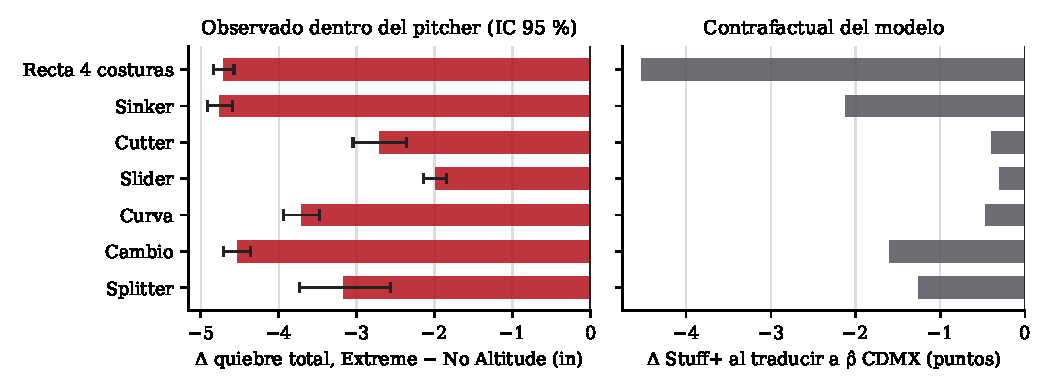
\includegraphics[width=\linewidth]{generated/fig_h1.pdf}
\caption{Izquierda: pérdida de quiebre total observada dentro del mismo pitcher. Derecha: cambio de \splus\ que predice el modelo al llevar cada pitcheo de la LMB a la densidad de la CDMX. Coinciden en los extremos (rectas castigadas, slider resistente), no en el orden intermedio: el sinker y el cambio pierden casi tanto quiebre como la recta, pero el modelo les resta mucho menos \splus.}\label{fig:h1}
\end{figure}

El contrafactual del modelo coincide con lo observado solo en los extremos (Figura~\ref{fig:h1}). Al traducir cada pitcheo de la LMB de $\rho=1$ a $\rhohat_{\text{CDMX}}$, la recta pierde en promedio \cf{cf.fourseam.delta.abs} puntos de \splus\ y el sinker \cf{cf.sinker.delta.abs}, mientras que slider (\cf{cf.slider.delta}), cutter (\cf{cf.cutter.delta}) y curva (\cf{cf.curveball.delta}) casi no cambian (Tabla~\ref{tab:cf}). El orden intermedio no coincide: el sinker pierde más quiebre observado que la recta (\cf{h1.sinker.tib} frente a \cf{h1.fourseam.tib}~in), pero el modelo le resta menos de la mitad, y el cambio pierde \cf{h1.changeup.tibabs}~in con solo \cf{cf.changeup.delta} puntos. El modelo no valora igual cada pulgada de quiebre en todas las familias. En el leaderboard (\cf{lb.n} temporadas de pitcher con al menos \cf{lb.min} pitcheos), el $\Delta\splus_{\text{CDMX}}$ correlaciona $r=\cf{lb.corr.fsuso}$ con el uso de la recta de cuatro costuras.

\begin{table}[htbp]\centering\small
\caption{Contrafactual del modelo: \splus\ medio ponderado por pitcheos al traducir cada lanzamiento del sabor neutral al CDMX.}\label{tab:cf}
\tabla{tab_contrafactual}
\end{table}

\paragraph{H2, resiliencia: consistente con el modelo, no con lo observado.} Definimos el grupo resiliente como cambio y splitter, y el aerodinámico como recta de cuatro costuras, curva y slider (el sinker y el cutter quedan fuera). Dentro del mismo pitcher, el contrafactual de \splus\ resta \cf{h2.est} puntos menos al grupo resiliente (IC 95\% \cf{h2.ci}, $n=\cf{h2.n}$). Pero los datos observados no respaldan H2 para el cambio: pierde \cf{h1.changeup.tibabs}~in de quiebre total, casi lo mismo que la recta, y su whiff cae \cf{h1.changeup.whiff.abs}~pp, la mayor caída significativa de todas las familias. Además, el slider, que pertenece al grupo aerodinámico, es el más resistente en las dos vistas. La frontera útil no es ``gravedad contra giro''.

\paragraph{H3, valor de los rodados: no confirmada.} Entre \cf{h3.n} pitchers con muestra en ambos entornos, su tasa basal de rodados no predice cuánto valor pierden en altitud (pendiente \cf{h3.est}, IC \cf{h3.ci}, $p=\cf{h3.p}$) ni cuánto sube su tasa de HR ($p=\cf{h3.hr.p}$). La intuición física es razonable, pero con estos datos no podemos sostenerla.

\paragraph{H4, forma frente a spin bruto: no confirmada.} En una regresión conjunta dentro de \emph{Extreme Altitude} ($n=\cf{h4.n}$ pitchers, bootstrap por pitcher), la única variable significativa para el valor en carreras es el \texttt{SpinRate} bruto ($p\cf{h4.xrv.spin.prel}$). La eficiencia de giro (\texttt{SpinToBreakRatio}, $p\cf{h4.xrv.s2b.prel}$) y el movimiento observado no lo son. Para whiff, \texttt{SpinRate} ($p\cf{h4.whiff.spin.prel}$) y \texttt{SpinToBreakRatio} ($p\cf{h4.whiff.s2b.prel}$) son significativos, pero el signo de la eficiencia es negativo. Es una regresión transversal entre pitchers dentro de \emph{Extreme}, sin comparación con \emph{No Altitude}: muestra que, en altitud, más spin se asocia con más valor, no que el spin proteja \emph{más} en altitud que al nivel del mar, ni que lo cause.

\begin{table}[htbp]\centering\small
\caption{H4: regresión conjunta en \emph{Extreme Altitude} con IC bootstrap por pitcher.}\label{tab:h4}
\tabla{tab_h4}
\end{table}

\paragraph{Descomposición en canales.} Dentro de \cf{canal.n} pitchers, el valor por pitcheo cae \cf{canal.total.per100.abs} carreras por cada 100 lanzamientos en \emph{Extreme} (IC \cf{canal.total.ci} por pitcheo). Lo separamos en tres términos:
\begin{itemize}
  \item \textbf{Canal Stuff} (\cf{canal.stuff.share}\%, \cf{canal.stuff.per100} carreras por 100): contrafactual del propio modelo \splus\ en las mismas filas a dos densidades. Es lo que la altitud le quita al pitcheo.
  \item \textbf{Canal parque} (\cf{canal.park.share}\%, \cf{canal.park.per100} carreras por 100): diferencia de valor en pelotas en juego condicionada a la velocidad y el ángulo de salida. Es la misma calidad de contacto, que en altitud produce más daño.
  \item \textbf{Residuo no atribuido} (\cf{canal.unallocated.share}\%, \cf{canal.unallocated.per100} carreras por 100). No lo asignamos a ningún canal: incluye cambios de ubicación, de selección de pitcheos y de bateadores entre ambos entornos.
\end{itemize}
La lectura operativa: de lo que sí podemos atribuir, el canal parque es \cf{canal.ratio} veces mayor que la pérdida física de los pitcheos. Por eso el sabor CDMX de \splus\ solo descuenta el canal Stuff.

%=====================================================================
\section{Aplicabilidad y fronteras del modelo}
\label{sec:aplicacion}

\paragraph{Herramientas.} El \textbf{simulador} (Streamlit) recibe las características de un pitcheo, lo traduce a ambas densidades y muestra \splus, \lplus\ y \pplus\ lado a lado, la atribución SHAP y el mapa de movimiento. El \textbf{Pitch Sculptor} no inventa pitcheos: busca, entre pitchers reales con el mismo slot ($\pm\cf{sc.slot.tol}^\circ$), altura de soltura ($\pm\cf{sc.relh.tol}$~ft) y velocidad de recta ($\pm\cf{sc.velo.tol}$~mph), qué formas logran más \splus\ CDMX, y reporta el rango intercuartílico de las filas más cercanas de esa familia en mecánica. Si hay menos de cinco pares, no emite recomendación. \textbf{VeloVision} estima el slot de brazo desde video de bullpen y devuelve un \emph{rango} de \splus\ CDMX por familia, a partir de los pitchers del dataset con slot similar; nunca da un valor puntual.

\paragraph{Fronteras y limitaciones (las declaramos antes de que nos las pregunten).}
\begin{itemize}
  \item \splus\ casi no predice el valor en carreras de un pitcheo aislado (Sección~\ref{sec:val}). Debe usarse como descriptor físico, no como pronóstico.
  \item La estabilidad entre años reportada es dentro de muestra.
  \item \emph{Extreme Altitude} mezcla varios parques: el sabor CDMX usa su mediana ($\rhohat=\cf{rho.cdmx}$), no una medición del Harp Helú.
  \item El \cf{canal.unallocated.share}\% del efecto total queda sin atribuir, y el canal parque es un contraste condicionado, no un efecto causal.
  \item H3 y H4 no se confirman, H1 se confirma solo para las rectas y H2 solo en el contrafactual del modelo.
  \item No hay orientación de costura, así que la estela desplazada por la costura no es modelable. Tampoco hay corredores en base, así que el valor en carreras usa outs $\times$ conteo.
  \item Las comparaciones dentro del mismo pitcher controlan la identidad del pitcher, pero no la selección del rival ni del bateador en cada parque.
  \item VeloVision mide la altura de soltura desde el tobillo del pie de apoyo y no desde el nivel del campo como TrackMan. Ese sesgo de origen no está medido, y la validación con anotadores humanos no lo detecta porque ambos miden en el mismo video. Por eso entrega rangos amplios y debe considerarse experimental.
  \item Los IDs son anónimos y no hay equipo en los datos, así que no podemos identificar el staff de Diablos. Las recomendaciones se expresan por perfil.
\end{itemize}

\paragraph{Reproducibilidad.} Todo el pipeline es determinista y está cubierto por pruebas automáticas. Todas las cifras de este documento se generan desde \texttt{reports/} con \texttt{analysis/build\_paper\_numbers.py}; ningún número está escrito a mano.

\end{document}
